%compile with pdflatex on papeeria

\documentclass[a4paper,12pt]{article}
\usepackage{fancyhdr}
\usepackage{fancyheadings}
\usepackage[ngerman,german]{babel}
\usepackage{german}
\usepackage[utf8]{inputenc}
%\usepackage[latin1]{inputenc}
\usepackage[active]{srcltx}
%\usepackage{algorithm}
%\usepackage[noend]{algorithmic}
\usepackage{amsmath}
\usepackage{amssymb}
\usepackage{amsthm}
\usepackage{bbm}
\usepackage{enumerate}
\usepackage{graphicx}
\usepackage{ifthen}
\usepackage{listings}
\usepackage{enumitem}
%\usepackage{struktex}
\usepackage{hyperref}
\usepackage{tikz}
\usepackage{float}
\usepackage{subcaption}
\captionsetup{compatibility=false}
\captionsetup[subfigure]{labelformat=empty}

\usepackage{pgfplots}
\usepgfplotslibrary{fillbetween}
%\usetikzlibrary{patterns}
\pgfplotsset{compat=1.15}
\usepackage{mathrsfs}
\usetikzlibrary{arrows}

\pgfplotsset{grid style={dashed,gray}}

\definecolor{ccqqqq}{rgb}{0.8,0,0}

\pagenumbering{gobble}

%%%%%%%%%%%%%%%%%%%%%%%%%%%%%%%%%%%%%%%%%%%%%%%%%%%%%%
%%%%%%%%%%%%%% EDIT THIS PART %%%%%%%%%%%%%%%%%%%%%%%%
%%%%%%%%%%%%%%%%%%%%%%%%%%%%%%%%%%%%%%%%%%%%%%%%%%%%%%
\newcommand{\Fach}{1. Klausur aus der Mathematik (A)}
\newcommand{\Name}{}
\newcommand{\datum}{}
\newcommand{\Matrikelnummer}{}
\newcommand{\Semester}{Q12/1}
\newcommand{\Uebungsblatt}{} %  <-- UPDATE ME
%%%%%%%%%%%%%%%%%%%%%%%%%%%%%%%%%%%%%%%%%%%%%%%%%%%%%%
%%%%%%%%%%%%%%%%%%%%%%%%%%%%%%%%%%%%%%%%%%%%%%%%%%%%%%

\setlength{\parindent}{0em}
\topmargin -1.0cm
\oddsidemargin 0cm
\evensidemargin 0cm
\setlength{\textheight}{9.2in}
\setlength{\textwidth}{6.0in}

%%%%%%%%%%%%%%%
%% Aufgaben-COMMAND
\newcommand{\Aufgabe}[1]{
  {
  \vspace*{0.5cm}
  \textsf{\textbf{Aufgabe #1}}
  \vspace*{0.2cm}
  
  }
}
%%%%%%%%%%%%%%
\hypersetup{
    pdftitle={\Fach{}: Übungsblatt \Uebungsblatt{}},
    pdfauthor={\Name},
    pdfborder={0 0 0}
}

\lstset{ %
language=java,
basicstyle=\footnotesize\tt,
showtabs=false,
tabsize=2,
captionpos=b,
breaklines=true,
extendedchars=true,
showstringspaces=false,
flexiblecolumns=true,
}

\title{Übungsblatt \Uebungsblatt{}}
\author{\Name{}}

\begin{document}
\thispagestyle{fancy}
%\lhead{\sf \large \Fach{} \\ %\small \Name{} - \Matrikelnummer{}
\lhead{\sf \large \Fach{} %\small \Name{} - \Matrikelnummer{}
}
\rhead{\sf \Semester{}   \datum{}}
%\rhead{\sf \Semester{} }
\vspace*{0.2cm}
%\begin{center}
%%\LARGE \sf \textbf{Übungsblatt \Uebungsblatt{}}
%\end{center}
%\vspace*{0.2cm}

%%%%%%%%%%%%%%%%%%%%%%%%%%%%%%%%%%%%%%%%%%%%%%%%%%%%%%
%% Insert your solutions here %%%%%%%%%%%%%%%%%%%%%%%%
%%%%%%%%%%%%%%%%%%%%%%%%%%%%%%%%%%%%%%%%%%%%%%%%%%%%%%

  Name: \underline{\hspace{7cm}}
%\draw[line width=1pt,color=ccqqqq,smooth,samples=100,domain=-6:7] plot(\x,{(1/12)*\x*\x+(1/3)*\x});
  \hfill
  Datum: \underline{\hspace{4cm}}

%\vspace{0,5cm}Die Rechenwege müssen nachvollziehbar sein!

\vspace{0,5cm} {TEIL A} - ohne Hilfsmittel
\vspace {0,2cm}
 

\Aufgabe{1} 
Gegeben ist der Graph einer Funktion $f$(s. unten). Bestimmen Sie, ob die Aussagen wahr oder falsch sind. Begründen Sie jeweils Ihre Antwort:

\begin{enumerate}[label={\alph*)}]
  \item $F$ hat 3 Extrema
  \item $F$ hat 3 Wendepunkte
  \item $f'$ hat zwei Nullstellen
  \item $f'(1)=0$
  \item $f(2)=0$
  \item $f'(2)=0$
  \item $f'(-1)<0$
\end{enumerate}


\begin{figure}[H]
\centering
  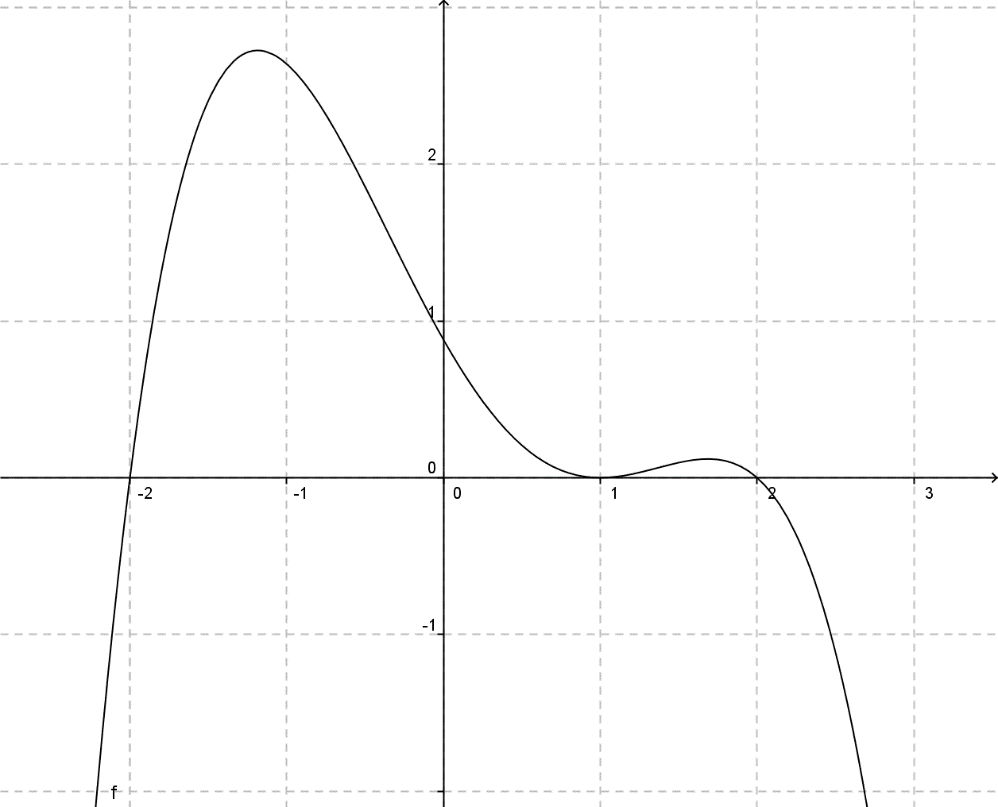
\includegraphics{210227.png}
\end{figure}

\newpage

\Aufgabe{2:} 
Bestimmen Sie folgende Integrale

\begin{enumerate}[label={\alph*)}]
  \item $ \int \frac{-x^3-3x^2}{x^4+4x^3}\, dx$
  \item $ \int_{-1}^{1} -2x^2 +2x + 2 \, dx$
\end{enumerate}
%\begin{flushright}4 BE \end{flushright}

\Aufgabe{3:}
Gegeben ist eine Zufallsgröße $X$, die die Werte $x_i = \{-2; 0; 2; 4\}$ annimmt.\\
Dem untenstehenden Histogramm kann man die Wahrscheinlichkeitswerte $P(X = x_i)$ entnehmen



\begin{figure}[h!]
  \centering
\begin{tikzpicture}[>=latex, line cap=round, line join=round,>=triangle 45]
\begin{axis}[
  %unit vector ratio=1 10,
  axis x line=center,
  axis y line=center,
  axis line style = thick,
  xtick align=inside,
  %extra x tick style={tick style={very thick}}
  xtick={-4,-2,0,2,4},
  ytick={0,0.1,0.2,0.3,0.4},
  xtick style=thick,
  ytick style=thick,
  xticklabels={,,},
  extra x ticks={-2,0,2,4},
  bar width=1cm,
  %xticklabel style={anchor=south west},
  %minor x tick num=1,
  %minor y tick num=1,
  %minor tick num = 1,
  x=1cm,    %größe der kästchen in x-richtung
  y=10cm,    %größe der kästchen in y-richtung
  xlabel={$x$},
  ylabel={$P(X=x)$},
  ymajorgrids=true,
  xlabel style={below right},
  ylabel style={below right},
  %xmajorgrids=true,
  xmin=-4,
  xmax=5,
  ymin=0,
  ymax=0.4]

\addplot[ybar,fill=blue,fill opacity=0.2] coordinates {
        (-2,0.2)
        (0,0.3)
        (4,0.2)
    };
\end{axis}
\end{tikzpicture}
\end{figure}

%\begin{figure}[h!]
%  \centering
%  \includegraphics[width=0.5\columnwidth]{210227_barChart_p.png}
%\end{figure}

Ergänzen Sie den zu $x_i=2$ gehörenden Wahrscheinlichkeitswert im Histogramm und ermitteln Sie näherungsweise den Erwartungswert der Zufallsgröße.


\newpage
{TEIL B} - mit Hilfsmittel

\Aufgabe{4:}


\begin{enumerate}[label={\alph*)}]
  \item Die Abbildung zeigt den Graphen $G_f$  einer in $R$ definierten Funktion $f$ mit dem Wendepunkt $W(-1|2)$. Ermitteln Sie mithilfe der Abbildung näherungsweise den Wert der Ableitung von $f$  an der Stelle $x=-1$  und skizzieren Sie sodann den Graphen der Ableitungsfunktion $f'$  von $f$  in die Abbildung. Berücksichtigen Sie dabei insbesondere die Lage der Nullstellen von $f'$  sowie den für $f'(-1)$ ermittelten Näherungswert.

  \begin{figure}[H]
    \centering
    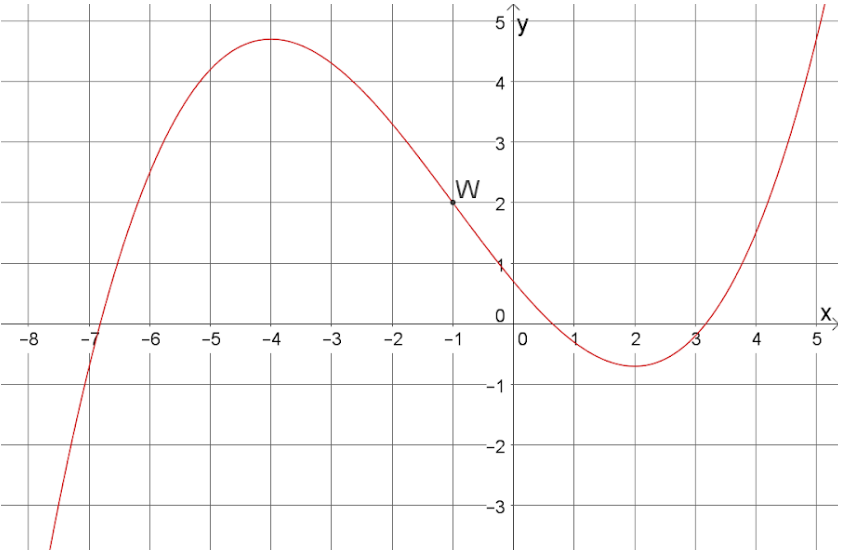
\includegraphics[width=0.8\columnwidth]{210227_funkcja.png}
    %\caption{A boat.}
    %\label{fig:boat1}
  \end{figure}

\item Betrachten Sie nun die Funktion $g: x\rightarrow e^{3x}-4$. Bestimmen Sie rechnerisch die Stelle, an der der Graph der Funktion die Steigung 6 hat.
\end{enumerate}


\Aufgabe{5:}
Gegeben sei die Funktion $f: x\rightarrow \frac{1}{2}x\cdot e^{-0.1x+2}$. Die Funktion hat bei $x=0$ ihre einzige Nullstelle.\\
Ihr Graph ist in der Abbildung dargestellt.\\
Die Funktion $F:x\rightarrow (-5x-50)\cdot e^{-0.1x+2}$ ist eine Stammfunktion der Funktion $f$.

\begin{figure}[H]
  \centering

    \subfloat[]{

\begin{tikzpicture}[>=latex, x=1cm, y=1cm, line cap=round, line join=round,>=triangle 45]
\begin{axis}[
  unit vector ratio=1 2,
  axis x line=center,
  axis y line=center,
  axis line style = thick,
  %extra x tick style={tick style={very thick}}
  xtick={-10,0,...,50,60},
  ytick={-10,-5,...,5,10},
  ticklabel style={fill=white},
  %extra x ticks={0},
  %xticklabel style={anchor=south west},
  %minor x tick num=1,
  %minor y tick num=1,
  %minor tick num = 1,
  %x=1cm,    %größe der kästchen in x-richtung
  %y=1cm,    %größe der kästchen in y-richtung
  xlabel={$x$},
  ylabel={$y$},
  grid=both,
  grid=major, grid style={dashed,gray!30},
  grid=minor, grid style={dashed,gray!30},
  ymajorgrids=true,
  xmajorgrids=true,
  xlabel style={below right},
  ylabel style={above left},
  xmin=-15.5,
  xmax=65.5,
  ymin=-10.5,
  ymax=14]
%\coordinate (O) at (0,0)
%\addplot [mark=none,domain=-15:15] {};
        \draw[line width=1pt,color=ccqqqq,smooth,samples=100,domain=-15:65] plot(\x,{0.5*\x*e^(-0.1*\x+2)});
  %\addplot[line width=1pt,color=ccqqqq, domain=-15:65]plot(\x,{0.5*\x*e^(-0.1*\x+2)});
\draw (26.07701146189816,9.323776772024983) node[anchor=north west] {$G_f$};

\end{axis}
\end{tikzpicture}

        %\addplot[line width=1pt,color=ccqqqq ]plot(\x,{0.5*\x*e^(-0.1*\x+2)});

%\draw (26.07701146189816,9.323776772024983) node[anchor=north west] {G_f};
%\begin{scriptsize}
%\draw[color=ccqqqq] (0.06341005665314936,-6.095192074225563) node {$f$};
%\end{scriptsize}
%\end{axis}
%\end{tikzpicture}

    }

\end{figure}


\begin{enumerate}[label={\alph*)}]
\item Bestimmen Sie das Krümmungsverhalten der Funktion $f$ sowie die Lage des Wendepunkts.\\
  \item Der Graph der Funktion $f$ und die $x$-Achse schließen im 1. Quadranten ein Flächenstück ein, das sich ins Unendliche ersreckt. Bestimmen Sie dessen Wert und interpretieren Sie diesen Wert geometrisch.
\end{enumerate}

\Aufgabe{6:}
In der dargestellten Abbildung sind die Graphen der Funktionen $f$ und $g$ mit $f(x)=\frac{1}{12}x^2+\frac{1}{3}x$ und $g(x)=\frac{1}{24}x^3-\frac{2}{3}x$ zu sehen.\\
Berechnen Sie den Inhalt der Fläche, die von den beiden Funktionsgraphen eingeschlossen wir. Die benötigten Schnittstellen sind ganzzahlig und dürfen aus der Abbildung abgelesen werden.


\begin{figure}[H]
  \centering

    \subfloat[]{

\begin{tikzpicture}[>=latex, x=1cm, y=1cm, line cap=round, line join=round,>=triangle 45]


\begin{axis}[
  %unit vector ratio=1 2,
  axis x line=center,
  axis y line=center,
  axis line style = thick,
  %extra x tick style={tick style={very thick}}
  xtick={-5,...,5,6},
  ytick={-2,-1,...,6},
  %extra x ticks={0},
  %xticklabel style={anchor=south west},
  minor x tick num=1,
  minor y tick num=1,
  %minor tick num = 1,
  x=1cm,    %größe der kästchen in x-richtung
  y=1cm,    %größe der kästchen in y-richtung
  xlabel={$x$},
  ylabel={$y$},
  grid=both,
  grid=major, grid style={dashed,gray!30},
  grid=minor, grid style={dashed,gray!30},
  %ticklabel style={fill=white},
  ymajorgrids=true,
  xmajorgrids=true,
  xlabel style={above left},
  ylabel style={below right},
  xmin=-5.5,
  xmax=6.5,
  ymin=-1.5,
  ymax=6,
  after end axis/.code={
        \path (axis cs:0,0) 
            node [anchor=north west,yshift=-0.075cm,xshift=-0.475cm] {0};
            %node [anchor=south west,xshift=-0.075cm] {0};
    }
]
%\coordinate (O) at (0,0)
  \addplot [name path=f, line width=1pt,color=ccqqqq,smooth,samples=100,domain=-6:7] {(1/12)*x^2+(1/3)*x} node [pos=0.8, above left] {$G_f$};
  %node[below,pos=1] {$Gf$};

  \addplot [name path=g, line width=1pt,color=ccqqqq,smooth,samples=100,domain=-6:7] {(1/24)*x^3-(2/3)*x} node [pos=0.7, below right] {$G_g$};

\addplot [
        thick,
        color=blue,
        fill=blue, 
        fill opacity=0.05,
        %pattern=north east lines
    ]
    fill between[
        of=f and g,
        soft clip={domain=-4:6},
    ];

   % \tikzfillbetween[
   %     of=f and g,split,
   %     every even segment/.style={pattern=crosshatch}
   %   ] {pattern=grid};
\end{axis}
\end{tikzpicture}

        %\addplot[line width=1pt,color=ccqqqq ]plot(\x,{0.5*\x*e^(-0.1*\x+2)});

%\draw (26.07701146189816,9.323776772024983) node[anchor=north west] {G_f};
%\begin{scriptsize}
%\draw[color=ccqqqq] (0.06341005665314936,-6.095192074225563) node {$f$};
%\end{scriptsize}
%\end{axis}
%\end{tikzpicture}

    }

\end{figure}

\Aufgabe{7:}
Der Kapitän der deutschen Handballnationalmannschaft Uwe Gensheimer hat bei 7-Meter-Würfen eine Trefferquote von 83\% (unabhängig von seiner Tagesform!).
\begin{enumerate}[label={\alph*)}]
  \item Im Training wirft Gensheimer 40-mal von der 7-Meter-Linie aufs Tor.\\
    Berechnen Sie die Wahrscheinlichkeit, dass Gensheimer genau 31-mal trifft!
  \item Im normalen Spielverlauf hat Gensheimer eine Trefferquote von 75\%.\\
    Berechnen Sie die Wahrscheinlichkeit, dass Gensheimer von insgesamt 100 Würfen über mehrere Spiele hinweg mindestens 70-mal und höchstens 80-mal trifft!
\end{enumerate}


\Aufgabe{8:}
Schon seit längerem halten sich Gerüchte über eine europäische „Superleague“, in der Europas Topvereine gegeneinander antreten. Diese Liga soll 20 Fußballclubs beinhalten.
\begin{enumerate}[label={\alph*)}]
  \item Bestimmen Sie die Anzahl der Spiele während einer Saison, wenn jedes Team gegen jedes Team genau zweimal spielt.\\

Nach dem Topspiel des Spieltags muss von jeder Mannschaft ein zufällig ausgewählter Spieler zur Dopingkontrolle. In Mannschaft A gibt es einen gedopten Spieler, in Mannschaft B gibt es zwei. Jede Mannschaft besteht aus 20 Spielern (Kadergröße). Die Zufallsgröße $X$  gibt die Anzahl der überführten Dopingsünder an.
  \item Berechnen Sie die Wahrscheinlichkeit, dass insgesamt genau ein gedopter Spieler ausgewählt wird.\\
    {[Ergebnis: 14\%]}
    \item Christiano berechnet den Erwartungswert der Zufallsgröße $X$ und erhält als Ergebnis 0,12.\\
Begründen Sie ohne explizite Berechnung des Erwartungswertes, dass Christiano falsch gerechnet hat!
\end{enumerate}


\Aufgabe{9:}
Eine ägyptische Pyramide hat die Form einer geraden quadratischen Pyramide. Die Seitenlänge des Grundquadrats beträgt 160m, die Höhe der Pyramide 100m. Im Modell in einem Koordinatensystem mit Längeneinheit 1m liegt der Ursprung genau in der Mitte der quadratischen Grundfläche und die $x_1$- und $x_2$-Achse verlaufen parallel zu den Grundkanten. 

  \begin{figure}[H]
    \centering
    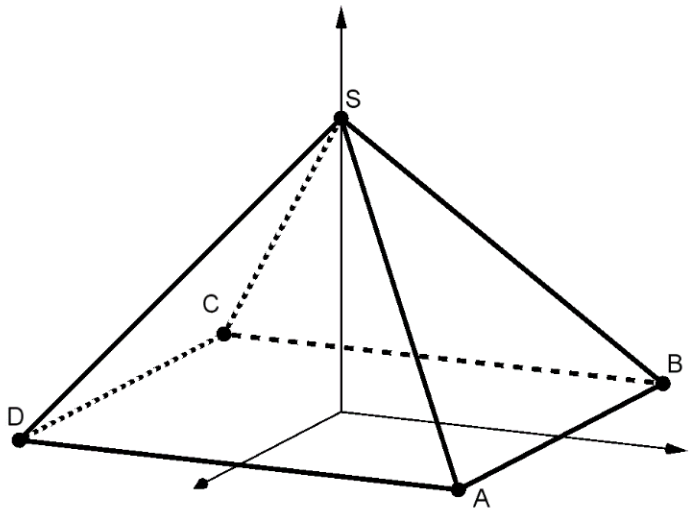
\includegraphics[width=0.5\columnwidth]{210227_pyramide.png}
    %\caption{A boat.}
    %\label{fig:boat1}
  \end{figure}




\begin{enumerate}[label={\alph*)}]
  \item Geben Sie die Koordinaten der Eckpunkte $A$,$B$ und $S$ an und bestimmen Sie die Gleichung der Ebene $E$ durch diese Punkte in Koordinatenform.\\
    {\it [mögliches Teilergebnis: $E: 5x_2 + 4x_3 = 400$]}
  \item Die Ägypter bauten die Pyramide schichtweise. Zum Transport der Steine zur jeweiligen Schicht wurde eine Rampe benötigt. Die Rampe führt enlang der Geraden\\

\[
\begin {aligned}
    r: \vec{X}= \begin{pmatrix} 0 \\
                              200 \\
                                0
                  \end{pmatrix}
           + \mu \begin{pmatrix} 0 \\
                                24 \\
                                -5
                  \end{pmatrix}
\end {aligned}
\qquad
\qquad
\raisebox{-10mm}{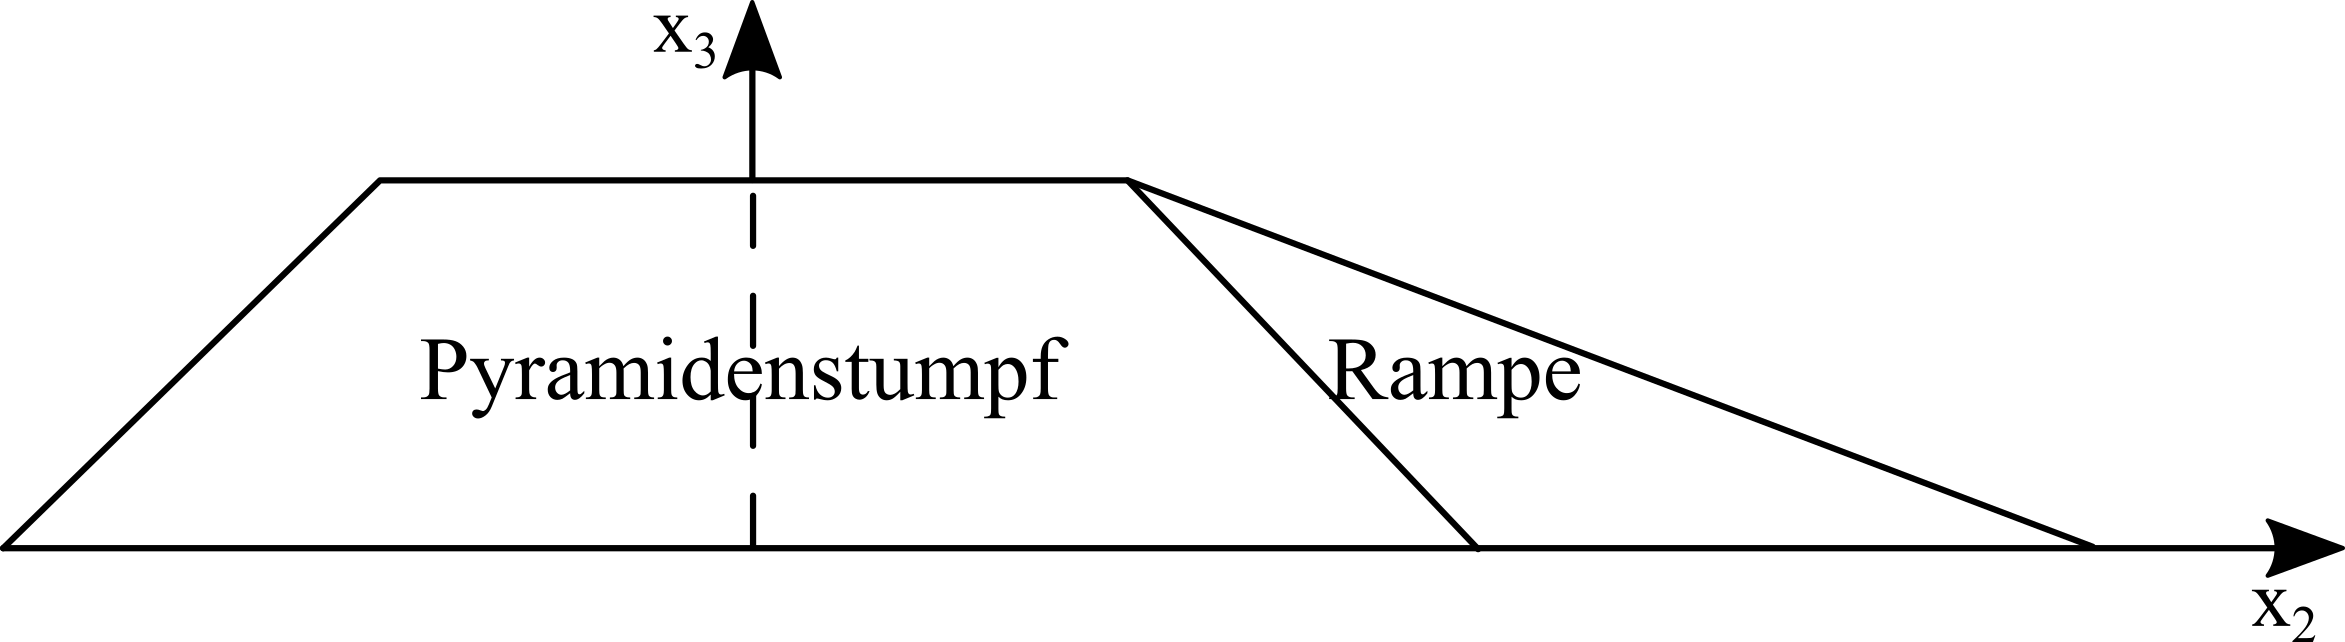
\includegraphics[keepaspectratio = true, scale = 0.5] {210227_pyramidenStumpfRampe.png}}
\]


  vom Erdboden bis an den Rand des bisher errichteten Pyramidenstumpfs und liegt in der $x_2-x_3$ Ebene.\\
    
    Berechnen Sie die Höhe des bisher gebauten Pyramidenstumpfes und die Länge der Rampe.\\

    Der Punkt $(0|60|25)$ liegt auf der Seitenfläche $ABS$. Er ist der Einstiegspunkt zu einem Schacht, der senkrecht zu dieser Seitenfläche verläuft und in 13m Höhe über der Grundfläche am Eingang der inneren Grabkammer endet. Berechnen Sie die Koordinaten dieses Endpunkts.
\end{enumerate}



\centerline{Viel Erfolg}
%\enlargethispage{2\baselineskip}

%\addtolength{\voffset}{-2cm}




%\begin{tikzpicture}
%\draw [very thin, black, step=0.5cm] (0,0) grid +(15,18);
%\end{tikzpicture}




%%%%%%%%%%%%%%%%%%%%%%%%%%%%%%%%%%%%%%%%%%%%%%%%%%%%%%
%%%%%%%%%%%%%%%%%%%%%%%%%%%%%%%%%%%%%%%%%%%%%%%%%%%%%%
\end{document}
